\documentclass[10pt,a4paper,twoside]{beamer}
\usepackage[spanish,activeacute]{babel}
\usepackage[utf8]{inputenc}
\usepackage{examplep}
\usepackage{subcaption}
\usepackage{fancyvrb}
\usepackage{adjustbox}

\mode<presentation> {
\usetheme{Madrid}
}

%----------------------------------------------------------------------------------------
%	PÁGINAS INCIALES
%----------------------------------------------------------------------------------------

\title[Modelización de series temporales]{Modelización de series temporales: aplicaciones en $\textsf{R}$} 
\date{19 de Julio, 2017} 
\author[Jose González Abad]{Autor: Jose González Abad\\Tutora: Rosa Sepúlveda Correa}
\institute[USAL]
{
Universidad de Salamanca \\ 

\begin{figure}
    \centering
    \centerline{
\includegraphics[scale = 0.5]{Images/usal800.jpg}}
    \label{usal}
\end{figure}
}

\begin{document}

\newenvironment{itemize*}
        {\begin{itemize}
            \setlength{\itemsep}{1pt}
            \setlength{\parsep}{3pt}
            \setlength{\parskip}{3pt}}
        {\end{itemize}}

\begin{frame}
\titlepage 
\end{frame}

\begin{frame}
\frametitle{Índice} 
\tableofcontents 
\end{frame}

%----------------------------------------------------------------------------------------
%	CUERPO DE LA PRESENTACIÓN
%----------------------------------------------------------------------------------------

%------------------------------------------------
\section{Objetivos}
%------------------------------------------------

\begin{frame}
\frametitle{Objetivos}
\begin{itemize*}
\item Introducción teórica el análisis de series temporales.
\item  Recorrido por librerías de $\textsf{R}$ orientadas a:
    \begin{itemize*}
    \item  Estructurar los datos.
    \item  Modelizar.
    \end{itemize*}
\item  Conclusiones.
    \begin{itemize*}
    \item Metodología para el análisis de series temporales en $\textsf{R}$.
    \end{itemize*}
\end{itemize*}

\end{frame}

%------------------------------------------------
\section{Conceptos generales}
%------------------------------------------------

\subsection{Enfoque determinista}

%------------------------------------------------

\begin{frame}
\frametitle{Enfoque determinista}

\begin{block}{Definición}
Supone que la serie temporal se puede expresar como la combinación de distintas componentes.
\begin{equation*}
    Y_{t} = f(t) + a_t \quad \text{con} \quad a_t \approx RB(0, \sigma^2)
\end{equation*}
\end{block}
\vspace{.5cm}
\begin{columns}[c]
\column{.5\textwidth}
\textbf{Componentes}
\begin{itemize*}
\item \textbf{Tendencia} ($T_t$): Evolución de la serie a largo plazo.
\item \textbf{Estacionalidad} ($S_t$): Variaciones recurrentes en periodos de tiempo cortos.
\item \textbf{Ciclo} ($C_t$): Variaciones recurrentes en periodos de tiempo largos.
\item \textbf{Fluctuaciones irregulares} ($a_t$): Fluctuaciones con apariencia no determinística.
\end{itemize*}

\column{.5\textwidth}
\textbf{Estructura}
\begin{itemize*}
\item \textbf{Aditiva}:
      \begin{equation*}
        Y_t = T_t + S_t + C_t + a_t
      \end{equation*}
\item \textbf{Multiplicativa}:
      \begin{equation*}
        Y_t = T_t \times S_t \times C_t \times a_t
      \end{equation*}
\end{itemize*}
\end{columns}

\end{frame}

%------------------------------------------------

\begin{frame}

\textbf{Estimación de las componentes}\\

\begin{itemize*}
\item \textbf{Estimación de la Tendencia}
    \begin{itemize*}
    \item Ajuste de funciones a la tendencia (lineal, exponencial...).
    \item Método de la media móvil:
        \begin{equation*}
        Y'_{t} = \frac{1}{p}\left(Y_{t-\left(\frac{p-1}{2}\right)}+...+Y_{t-1}+Y_t+Y_{t+1}+...+Y_{t+\left(\frac{p-1}{2}\right)}\right)
        \end{equation*}
    \end{itemize*}
\item \textbf{Estimación del ciclo}: Esta componente es difícil de estimar. Se suele incluir junto a la tendencia.
\item \textbf{Estimación de la estacionalidad}:
    \begin{itemize*}
    \item Ajuste de funciones periódicas a la estacionalidad.
    \item Variables \textit{dummy}:
        \begin{equation*}
        g(t) = \sum_{i=1}^{S}(\lambda_{i} d_{it})
        \end{equation*}
    \end{itemize*}
\item \textbf{Estimación de la componente irregular}:
\begin{equation*}
    Y_t - T_t - S_t - C_t = a_t
\end{equation*}
\begin{equation*}
    \frac{Y_t}{T_t \times S_t \times C_t} = a_t
\end{equation*}
\end{itemize*}

\end{frame}

%------------------------------------------------

\begin{frame}
\vspace{.5cm}

    \begin{columns}[t]
        \column{.5\textwidth}
        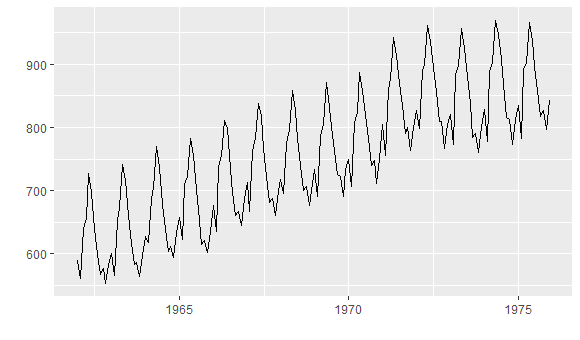
\includegraphics[width=\columnwidth,height=3cm]{Images/serie.png}
        \captionof{figure}{Serie original}
        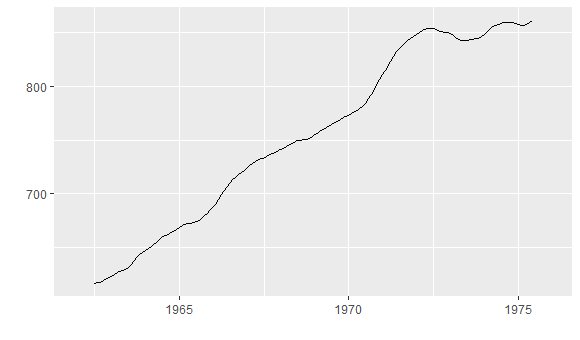
\includegraphics[width=\columnwidth,height=3cm]{Images/tend.png}
        \captionof{figure}{Tendencia}
        \column{.5\textwidth}
        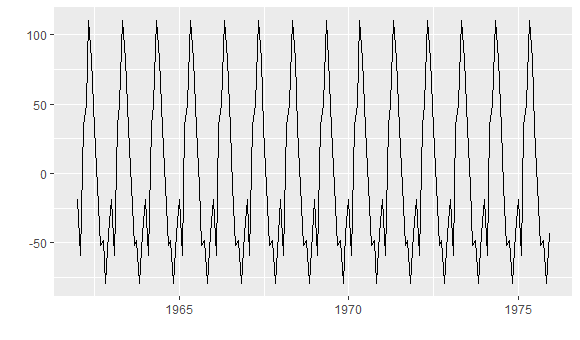
\includegraphics[width=\columnwidth,height=3cm]{Images/season.png}
        \captionof{figure}{Estacionalidad}
        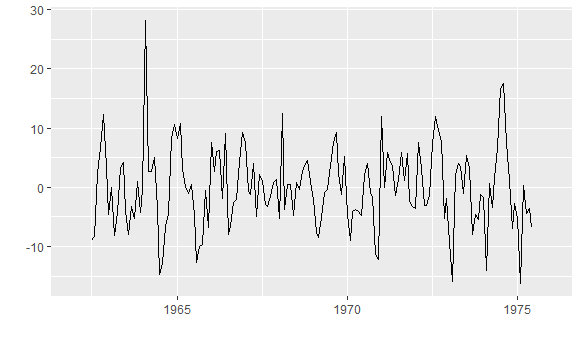
\includegraphics[width=\columnwidth,height=3cm]{Images/random.png}
        \captionof{figure}{Componente irregular}
    \end{columns}

\end{frame}

%------------------------------------------------

\subsection{Metodología Box-Jenkins}

%------------------------------------------------

\begin{frame}
\frametitle{Metodología Box-Jenkins}

\begin{block}{Definición}
Supone que la serie temporal es la realización de un proceso estocástico determinado y modelizable. Se sustenta en los modelos ARIMA.
\end{block}

\vspace{0.3cm}

\vspace{0.5cm}
\begin{block}{Estacionariedad débil}
Para trabajar con esta familia de modelos es necesario trabajar bajo los siguientes supuestos:
\begin{equation*}
    E[Y_{t}]=\mu<\infty \quad \quad \forall{t}
\end{equation*}
\begin{equation*}
   Var(Y_{t})=\sigma^2<\infty \quad \quad \forall{t}
\end{equation*}
\begin{equation*}
    Cov(Y_{t},Y_{t+k})=E[(Y_{t}-\mu)(Y_{t+k}-\mu)]<\infty \quad \quad \forall{t}
\end{equation*}
\end{block}

\vspace{-0.2cm}

\vspace{0.15cm}

\end{frame}

%------------------------------------------------

\begin{frame}
\textbf{Modelos ARIMA}\\
Suponen que la serie en un momento $t$ depende de sus valores pasados hasta el rezago $t-p$, de su innovación contemporánea y de las pasadas hasta el rezago $t-q$:
\begin{equation*}
    Y_{t} = a_{t} + \sum_{i=1}^{p} \phi_{i} Y_{t-i} + \sum_{i=1}^{q} (-\theta_{i}) a_{t-i}
\end{equation*}
En términos del operador de retardos se puede expresar como:
\begin{equation*}
    \phi_{p}(L)Y_{t} = \theta_{q}(L)a_{t}
\end{equation*}
La serie no es estacionaria si la parte autorregresiva posee alguna raíz unitaria ($d$):
\begin{equation*}
\phi_{p}(L)Y_{t} = \gamma_{p-d}(L)\cdot(1-L)^{d}
\end{equation*}
Para solucionar esto se diferencia la serie $d$ veces:
\begin{equation*}
\gamma_{p-d}(L)\cdot\Delta^{d}Y_{t}=\theta_{q}(L)a_{t}
\end{equation*}

\end{frame}

%------------------------------------------------

\begin{frame}

\begin{itemize*}
\item \textbf{Preparación de los datos}: Buscamos que nuestra serie sea estacionaria tanto en tendecia como en varianza.
    \begin{itemize*}
    \item Estacionariedad en tendencia: Diferenciamos la serie $d$ veces, hasta conseguir estacionariedad.
    \item Estacionariedad en varianza: Estabilizamos la serie con logaritmos o transformación Box-Cox
    \end{itemize*}
\item \textbf{Identificación y selección del modelo}: Nuestro objetivo es encontrar los valores óptimos de $p$ y $q$. Para ello debemos estudiar la evolución de la función de autocorrelación y compararla con la teórica de los distintos modelos.
\item \textbf{Estimación de los parámetros}: Método de máxima verosimilitud, mínimos cuadrados no lineales...
\item \textbf{Validación del modelo}: Comprobamos si el ajuste de nuestro modelo es efectivamente el correcto. Para ello podemos estudiar:
    \begin{itemize*}
    \item Distribución y correlaciones de los residuos
    \item Significativadad de los coeficientes
    \item Poder predictivo
    \end{itemize*}
\item \textbf{Predicción}: Realizamos las predicciones para $Y_{t+h}$ con el modelo ajustado y validado.
\end{itemize*}

\end{frame}

%------------------------------------------------
\section{Estructura de los datos temporales en R}
%------------------------------------------------

\begin{frame}[fragile]
\frametitle{Estructura de los datos temporales en $\textsf{R}$}

Este tipo de datos necesitan clases especiales para el correcto tratamiento, no podemos recurrir al \PVerb{data.frame} clásico.\\
\vspace{0.2cm}
\textbf{Librería \PVerb{stats}}
\begin{itemize*}
\item Con la librería \PVerb{stats} es posible definir objetos de clase \PVerb{ts}.
\begin{Verbatim}[fontsize=\footnotesize]
    ts(data = NA, start = 1, end = numeric(), frequency = 1, ...)
\end{Verbatim}
\item Además de otros métodos enfocados a otras tareas:
    \begin{itemize*}
    \item \PVerb{plot.ts()} para representar gráficamente estos objetos.
    \item \PVerb{cbind()} para agrupar varias series en un mismo objeto.
    \item \PVerb{window()} para seleccionar fácilmente un subconjunto de la serie.
    \end{itemize*}
\end{itemize*}

\begin{figure}
    \centering
    \centerline{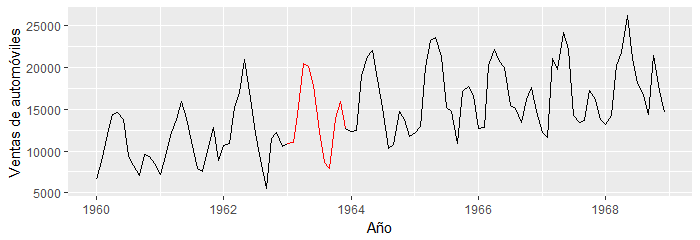
\includegraphics[scale = 0.4]{Images/window.png}}
    %\caption{}
    \label{window}
\end{figure}

\end{frame}

%------------------------------------------------

\begin{frame}[fragile]
\textbf{Librería \PVerb{zoo}}

\begin{itemize*}
\item Esta clase de objetos nos permite una estructuración más avanzada de series temporales. Se adaptan a periodos temporales irregulares.
    \begin{Verbatim}[fontsize=\footnotesize]
    zoo(x = NULL, order.by = index(), frequency = NULL)
    \end{Verbatim}
\item Métodos como \PVerb{index()}, \PVerb{coredata()} y \PVerb{merge.zoo()} nos facilitan la tarea de trabajar con la clase \PVerb{zoo}.
\item Esta librería incluye métodos muy potentes para el tratamiento de \PVerb{NAs}:
    \begin{itemize*}
    \item \PVerb{na.approx()}: recurre a interpolaciones lineales.
    \item \PVerb{na.spline()}: recurre a interpolaciones cúbicas de splines.
    \item \PVerb{na.locf()}: utiliza valores cercanos al valor faltante.
    \end{itemize*}
\item El método \PVerb{rollapply()} nos permite aplicar funciones a subconjuntos sucesivos de la serie.
    \begin{Verbatim}[fontsize=\footnotesize]
    rollapply(data, width, FUN, align)
    \end{Verbatim}
\item El método \PVerb{rollmean()} aplica un suavizado de medias móviles a nuestra serie. Es un implementación más directa del anterior.
\end{itemize*}

\end{frame}

%------------------------------------------------

\begin{frame}[fragile]
\textbf{Librería \PVerb{xts}}

\begin{itemize*}
\item Define la clase \PVerb{xts}, la cual se deriva de \PVerb{zoo}.
    \begin{Verbatim}[fontsize=\footnotesize]
    xts(x = NULL, order.by = index(x), frequency = NULL, unique = TRUE,…)
    \end{Verbatim}
\item Esta clase implementa una conversión más potente entre clases a través de \PVerb{as.xts()}.
\item Implementa una selección muy intuitiva de observaciones a través de fechas.
    \begin{Verbatim}[fontsize=\footnotesize, numbers = left]
    # diciembre de 1963
    xts.sales["1963-12"]
    # el año completo de 1963
    xts.sales["1963"]
    # todas las observaciones hasta julio de 1963
    xts.sales["/1963-7"]
    # todas las observaciones a partir de julio de 1963
    xts.sales["1963-7/"]
    # observaciones comprendidas entre julio de 1962 y de 1963
    xts.sales["1962-7/1963-7"]
    \end{Verbatim}
\item El método \PVerb{period.apply()} realiza una función similar al \PVerb{rollapply()} de \PVerb{zoo}.
\end{itemize*}

\end{frame}

%------------------------------------------------
\section{Modelización de series temporales con R}
%------------------------------------------------

\begin{frame}
\frametitle{Modelización de series temporales con R}

\begin{itemize*}
\item Trabajaremos con la serie correspondiente al número mensual de accidentes de tráfico ocurridos en Ontario en el periodo 1969-1974
\item Dividiremos la serie en un conjunto de \textit{training} (1969-1973) y en uno de \textit{test} (1974).
\end{itemize*}

\begin{figure}
    \centering
    \centerline{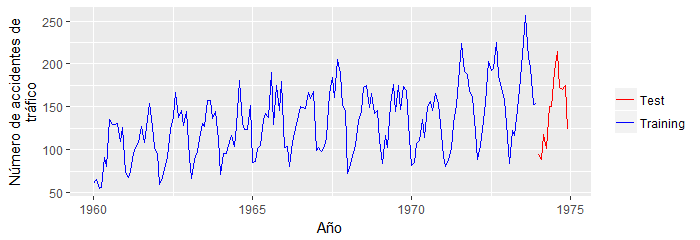
\includegraphics[scale = 0.6]{Images/31.png}}
    \label{accidentes}
\end{figure}

\end{frame}

%------------------------------------------------

\subsection{Forecast package}

%------------------------------------------------

\begin{frame}
\frametitle{Forecast package}
Esta librería está enfocada tanto al preprocesado como al análisis de series temporales univariantes. Trabajaremos con la clase \PVerb{ts}.\\
\vspace{0.3cm}

\begin{itemize*}
\item Para estudiar la estacionalidad más en detalle podemos recurrir al método \PVerb{seasonplot()}.
\end{itemize*}

\begin{figure}
    \centering
    \centerline{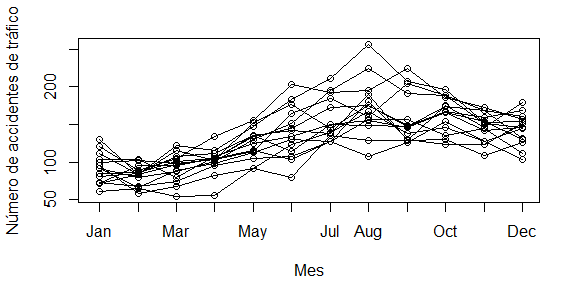
\includegraphics[scale = 0.6]{Images/32.png}}
    \label{season}
\end{figure}

\end{frame}

%------------------------------------------------

\begin{frame}
\textbf{Modelos ingenuos}\\
Con esta librería es posible ajustar varios modelos ingenuos a nuestros datos. Esto modelos nos pueden servir para trabajar bajo el principio de parsimonia.\\

\begin{itemize*}
\item \PVerb{meanf()}: Realiza predicciones con la media de la serie
\item \PVerb{naive()}: Predice con el valor anterior observado.
\item \PVerb{rwf()}: Variación de \PVerb{naive()} con pendiente.
\item \PVerb{snaives()}: Predice con el correspondiente valor estacional anterior.
\end{itemize*}

\vspace{0.5cm}

\begin{figure}
    \centering
    \centerline{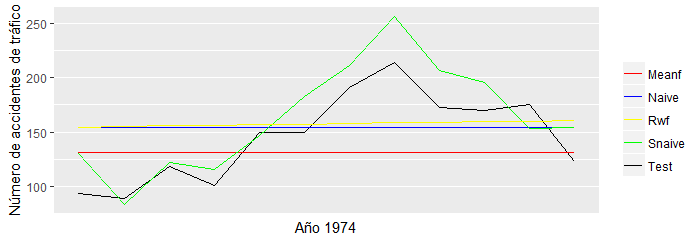
\includegraphics[scale = 0.5]{Images/311.png}}
    \label{comp}
\end{figure}

\end{frame}

%------------------------------------------------

\begin{frame}[fragile]
El método \PVerb{accuracy()} nos ofrece medidas de precisión del modelo en el conjunto de \textit{training} y \textit{test}. Si lo aplicamos sobre el modelo de \PVerb{meanf()} y el conjunto de \textit{test} \PVerb{acc.test} obtenemos lo siguiente:

\begin{Verbatim}[fontsize=\footnotesize]
                       ME     RMSE      MAE        MPE     MAPE     MASE
Training set 5.392491e-15 38.73302 31.48058 -10.085477 27.71539 1.774836
Test set     1.439286e+01 41.43521 36.28770   2.639993 25.15689 2.045855
                  ACF1 Theil's U
             0.7359523        NA
             0.6310518  1.205019
\end{Verbatim}

Para evaluar los modelos usaremos principalmente el MAE:
\begin{equation*}
    MAE = \frac{1}{T} \sum_{i = 1}^{n} \lvert Y_i - \widehat{Y}_i \lvert
\end{equation*}
El mejor MAE en el \textit{test} le obtenemos con \PVerb{snaive()} (22.58333).\\
Necesitamos ajustar modelos más complejos.

\end{frame}

%------------------------------------------------

\begin{frame}
\textbf{Modelo lineal}\\
El método \PVerb{tslm()} ajusta el siguiente modelo lineal:\\
\begin{equation*}
    Y_{t} = \beta_0 + \beta_1 t + \sum_{i = 2}^{M} \lambda_i d_i
\end{equation*}

Si lo aplicamos a nuestros obtenemos el siguiente modelo:\\
\begin{equation*}
    \widehat{Y}_{t} = 63.75 + 0.35 t - 9.99 d_2 - 0.06 d_3 + 8.72 d_4 + ... + 47.88 d_{12}
\end{equation*}

El MAE en el conjunto de \textit{test} es de 19.44597. Seguimos teniendo residuos con correlaciones significativas.\\

\begin{figure}
    \centering
    \centerline{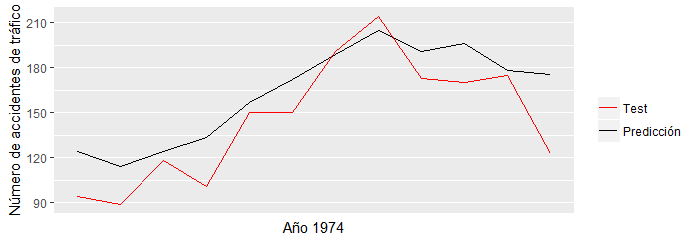
\includegraphics[scale = 0.5]{Images/312.png}}
\end{figure}

\end{frame}

%------------------------------------------------

\begin{frame}[fragile]
\textbf{Triple suavizado exponencial}\\
Este modelo realiza un suavizado exponencial a varias componentes para después combinarlas y realizar las predicciones.\\
A continuación se muestra el caso aditivo:
\begin{align*}
  \widehat{Y}_{t+h} &= l_t + h b_t + S_{t - M + h^+_M} \\
  l_t &= \alpha(Y_t - S_{t - M}) + (1 -\alpha)(l_{t-1}+ b_{t-1}) \\
  b_t &= \beta(l_t - l_{t-1}) + (1 -\beta) b_{t-1} \\
  S_t &= \gamma(Y_t - l_{t-1} + b_{t-1}) + (1 - \gamma) S_{t-M}
\end{align*}
Los coeficientes $\alpha$, $\beta$ y $\gamma$ determinan la importancia de las observaciones pasadas en la predicción.\\
Es posible añadir un parámetro $\phi$ de suavización o amortiguación de la tendencia (\textit{damped trend}).\\
Para ajustar este tipo de modelos recurrimos al método \PVerb{hw()}.\\

\vspace{.4cm}

\begin{Verbatim}[fontsize=\footnotesize]
hw(y, h = 2*frequency(x), seasonal = c("additive", "multiplicative"),
   damped = FALSE, initial = c("optimal", "simple"), alpha = NULL,
   beta =  NULL, gamma = NULL, phi = NULL, …)
\end{Verbatim}

\end{frame}

%------------------------------------------------

\begin{frame}[fragile]

\begin{figure}
    \centering
    \centerline{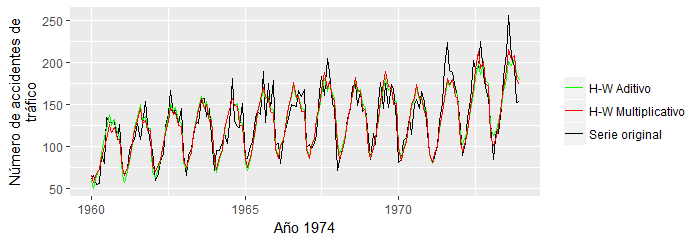
\includegraphics[scale = 0.5]{Images/313.png}}
\end{figure}

\begin{figure}
    \centering
    \centerline{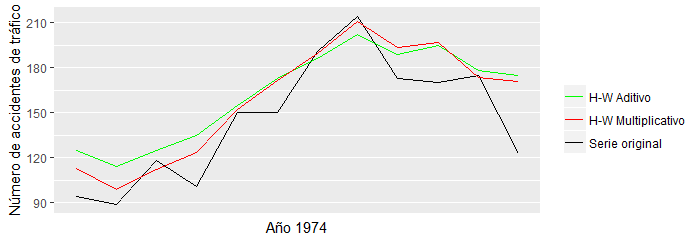
\includegraphics[scale = 0.5]{Images/314.png}}
\end{figure}

El MAE en estos modelos es de 19.67722 bajo estructura aditiva y 15.04762 bajo estructura multiplicativa.

\end{frame}

%------------------------------------------------

\begin{frame}
\textbf{Red neuronal}\\
Con el método \PVerb{nnetar()} es posible implementar una red NNAR$($p$, $P$, $k$)_M$ siendo:
\begin{itemize}
\item $p$ los rezagos que toma como \textit{inputs}.
\item $P$ los periodos anteriores de los que toma los valores correspondientes como \textit{inputs}.
\item $k$ el número de neuronas de la capa intermedia.
\end{itemize}

\begin{equation*}
    Y_{t-1}, Y_{t-2},...,Y_{t-p}, Y_{t-M}, Y_{t-2M},...,Y_{t-PM}
\end{equation*}

En este tipo de modelos el parámetro de regularización juega un papel fundamental ya que nos ayuda a controlar el \textit{overfitting}.
\begin{figure}
    \centering
    \centerline{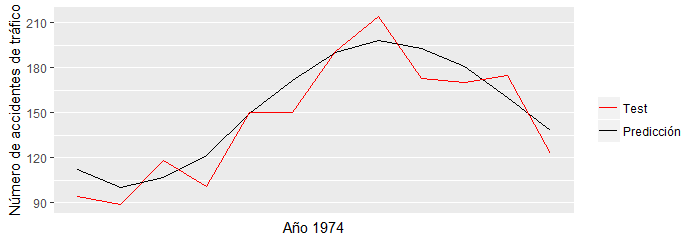
\includegraphics[scale = 0.4]{Images/317.png}}
\end{figure}

Obtenemos un MAE de 13.29118.

\end{frame}

%------------------------------------------------

\begin{frame}[fragile]
\textbf{Modelos ARIMA}\\
Esta librería implementa estos modelos a través de \PVerb{Arima()}.\\
\begin{Verbatim}
Arima(y, order = c(0,0,0), seasonal = c(0,0,0),
      include.mean = TRUE, include.drift = FALSE, …)
\end{Verbatim}

Para una selección óptima del modelo nos podemos apoyar en:
\begin{itemize*}
\item Análisis de la FAC y FACP a través de \PVerb{Acf()} y \PVerb{Pacf()}.
\item Determinar diferencias a partir de \PVerb{ndiffs()} y \PVerb{nsdiffs()}.
\end{itemize*}

Hemos optado por ajustar un SARIMA$(1,0,1)(2,1,1)_{12}$.

\begin{figure}
    \centering
    \centerline{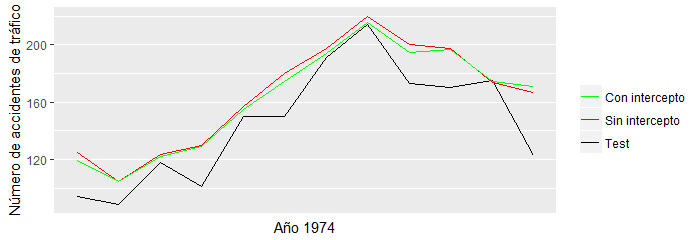
\includegraphics[scale = 0.5]{Images/320.png}}
\end{figure}

\end{frame}

%------------------------------------------------

\begin{frame}[fragile]
Es posible automatizar todo este proceso a través de \PVerb{auto.arima()}.
\begin{Verbatim}[fontsize=\footnotesize]
auto.arima(y, d = NA, D = NA, max.p = 5, max.q = 5, max.P = 2,
           max.Q = 2, max.d = 2, max.D = 1, ic = ("aicc", "aic", "bic"),
           test = c("kpss", "adf", "pp"),
           seasonal.test = c("ocsb", "ch"),...)
\end{Verbatim}
A través de sus argumentos es posible personalizar la búsqueda.

\begin{table}[]
\centering
\label{my-label}
\begin{adjustbox}{max width=\textwidth}
\begin{tabular}{|l|c|c|c|c|c|}
\hline
\multicolumn{1}{|c|}{}                & AIC              & AICc             & BIC & MAE & Ljung Box \\ \hline
$(0,1,0)(0,0,2)_{12}$               & 1550.38          & 1550.53          & 1559.73                  & 22.19949                 & $\sim 0$                                   \\ \hline
$(1,0,1)(2,1,1)_{12 \thinspace sin \thinspace int}$ & 1367.68          & 1368.25          & 1385.98                  & 19.22651                 & 0.04321                                  \\ \hline
$(1,0,1)(2,1,1)_{12 \thinspace con \thinspace int}$ & \textbf{1359.82} & \textbf{1360.58} & \textbf{1381.17}         & 17.09992                 & \textbf{0.2748}                          \\ \hline
$(1,0,0)(1,0,0)_{12}$               & 1514.22          & 1514.47          & 1526.72                  & \textbf{14.86938}        & 0.00085                                   \\ \hline
$(2,0,0)(2,0,0)_{12}$                & 1499.24          & 1499.77          & 1517.99                  & \textbf{14.96979}        & 0.002708                                  \\ \hline
$(1,1,4)(2,0,0)_{12}$               & 1485.29          & 1486.2           & 1510.24                  & 23.44705                 & 0.01353                                  \\ \hline
\end{tabular}
\end{adjustbox}
\end{table}

\end{frame}

%------------------------------------------------

\subsection{TSeries Package}

%------------------------------------------------

\begin{frame}
\frametitle{TSeries Package}
Necesitamos diferenciar y desestacionalizar la serie para trabajar con esta librería.

\begin{figure}
    \centering
    \centerline{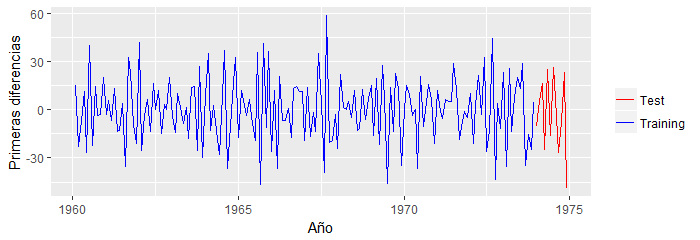
\includegraphics[scale = 0.5]{Images/323.png}}
\end{figure}

Parte del preprocesado se centra en la implementación de tests estadísticos:
\begin{itemize*}
\item Test aumentado de Dickey-Fuller (\PVerb{adf.test()})
\item Test de Philipps-Perron (\PVerb{pp.test()})
\item Test de KPSS (\PVerb{kpss.test()})
\item ...
\end{itemize*}

\end{frame}

%------------------------------------------------

\begin{frame}
\textbf{Técnicas de remuestreo}\\
Hay dos formas de implementar estas técnicas con esta librería:
\begin{itemize*}
\item \textbf{\PVerb{tsbootstrap()}}: implementa un \textit{bootstrap} por bloques. Existen dos variaciones:
    \begin{itemize*}
    \item \textbf{Por bloques}: La serie se divide en bloques de longitud $b$. Se hace un remuestreo aleatorio con reposición y se combinan respetando el orden temporal original.
    \item \textbf{Estacionario}: La longitud $b$ varía aleatoriamente.
    \end{itemize*}
\item \textbf{\PVerb{surrogate()}}: Recurre a transformadas de Fourier para generar remuestreos de la serie original.
\end{itemize*}

\begin{figure}
    \centering
    \centerline{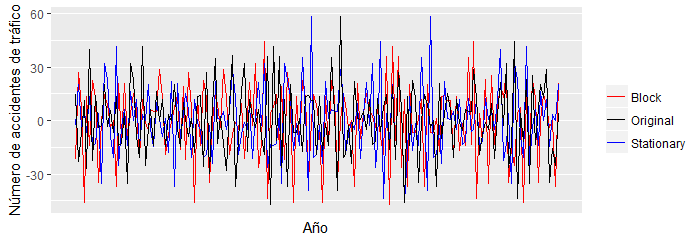
\includegraphics[scale = 0.6]{Images/32413242.png}}
\end{figure}

\end{frame}

%------------------------------------------------

\begin{frame}[fragile]
\textbf{Modelos ARMA}\\
Estos modelos se implementan a través de \PVerb{arma()}.

\begin{Verbatim}[fontsize=\footnotesize]
arma(x, order = c(1, 1), lag = NULL, coef = NULL,
     include.intercept = TRUE, qr.tol = 1e-07, ...)
\end{Verbatim}

Hemos ajustado un ARMA$(2,1)$.
\begin{figure}
    \centering
    \centerline{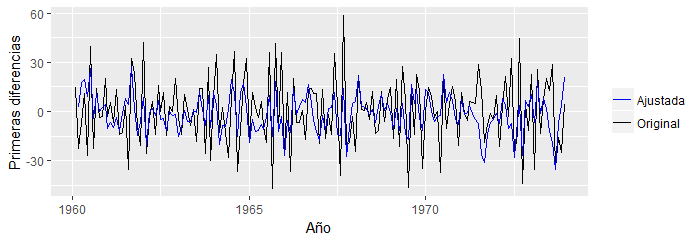
\includegraphics[scale = 0.6]{Images/3272.png}}
\end{figure}

Esta librería incluye métodos como \PVerb{jarque.bera.test()} y \PVerb{bds.test()} para estudiar lo residuos a través de tests estadísticos.

\end{frame}

%------------------------------------------------

\subsection{FitARMA Package}

%------------------------------------------------

\begin{frame}[fragile]
\frametitle{FitARMA Package}
Esta librería está enfocada a implementar modelos ARIMA.\\
Se caracteriza por utilizar un método de estimación que optimiza el ajuste del modelo.\\
Se implementa a través de \PVerb{FitARMA()}.
\begin{Verbatim}[fontsize=\footnotesize]
FitARMA(z, order = c(0, 0, 0), demean = TRUE, MeanMLEQ = FALSE,
        pApprox = 30, MaxLag = 30)
\end{Verbatim}

El parámetro \PVerb{pApprox} juega un papel fundamental en el ajuste.

\begin{figure}
    \centering
    \centerline{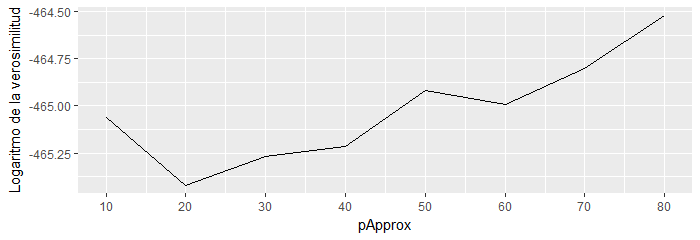
\includegraphics[scale = 0.5]{Images/330.png}}
\end{figure}

\end{frame}

%------------------------------------------------

\begin{frame}
Se ha llevado a cabo una simulación para estudiar el tiempo de ejecución de los métodos encargados de implementar los modelos ARMA/ARIMA de las tres librerías:
\begin{itemize*}
\item \PVerb{Arima()} de \PVerb{forecast}
\item \PVerb{arma()} de \PVerb{TSeries}
\item \PVerb{FitARMA()} de \PVerb{FitARMA}
\end{itemize*}

\begin{figure}
    \centering
    \centerline{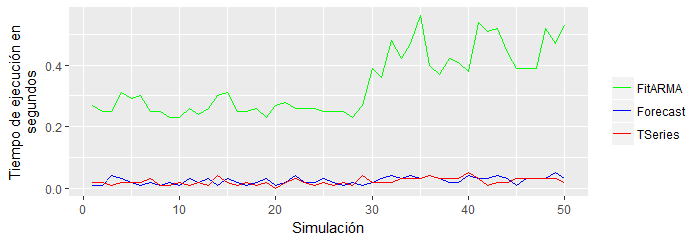
\includegraphics[scale = 0.6]{Images/331.png}}
\end{figure}

\end{frame}

%------------------------------------------------

\subsection{Opera Package}

%------------------------------------------------

\begin{frame}
\frametitle{Opera Package}
Esta librería nos permite combinar modelos a fin de obtener mejores predicciones.\\
\begin{equation*}
    \widehat{Y}_{t+h} = \sum_{k = 1}^{K} p_{k,t+h} \enskip  x_{k,t+h}
\end{equation*}
Hay dos formas de implementar esto:
\begin{itemize*}
\item \textbf{Combinaciones fuera de línea}: Se implementa a través de \PVerb{oracle()}. Ajusta las ponderaciones de acuerdo al poder predictivo de cada modelo. Es posible combinar las predicciones de dos formas:
    \begin{itemize*}
    \item Combinación lineal
    \item Combinación convexa
    \end{itemize*}
\end{itemize*}

\begin{figure}
    \centering
    \centerline{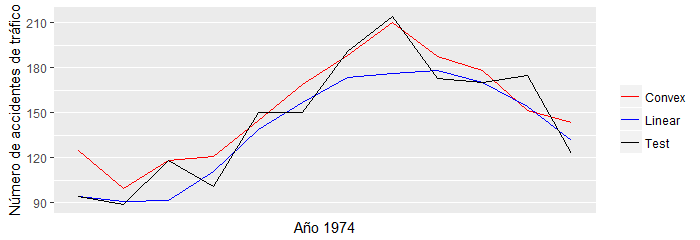
\includegraphics[scale = 0.5]{Images/336337.png}}
\end{figure}

\end{frame}

%------------------------------------------------

\begin{frame}

\begin{itemize*}
\item \textbf{Combinaciones en línea}: Implementa \textit{aggregation rules} a través de \PVerb{mixture()}. Son útiles para ajustar las ponderaciones secuencialmente.
\end{itemize*}

\begin{figure}
    \centering
    \centerline{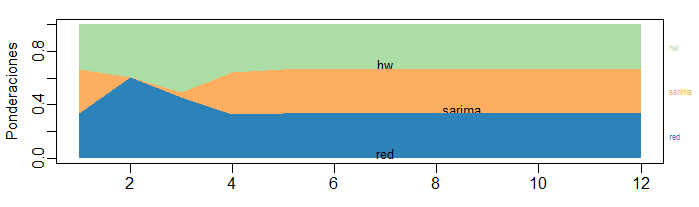
\includegraphics[scale = 0.5]{Images/338.png}}
\end{figure}

\begin{figure}
    \centering
    \centerline{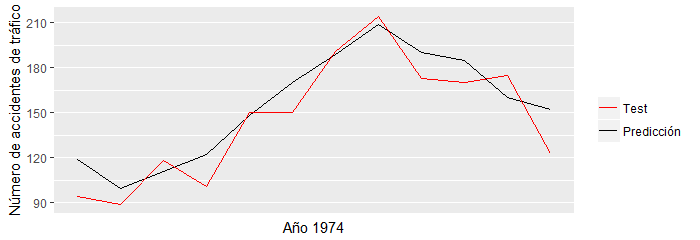
\includegraphics[scale = 0.5]{Images/337.png}}
\end{figure}

\end{frame}

%------------------------------------------------


%------------------------------------------------
\section{Conclusiones}
%------------------------------------------------

\begin{frame}
\frametitle{Conclusiones}

\begin{figure}
    \centering
    \centerline{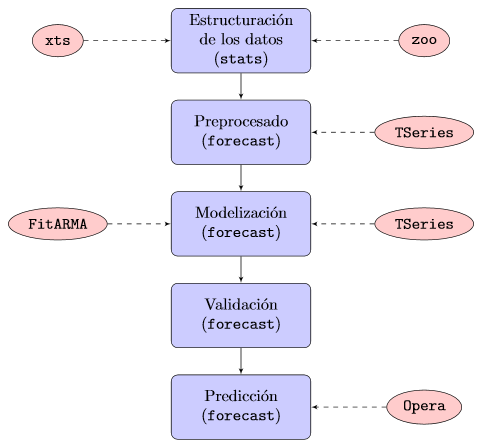
\includegraphics[scale = 0.5]{Images/esquema-conclusiones.png}}
\end{figure}

\end{frame}

%------------------------------------------------

\begin{frame}

\begin{center}
\Huge{Pero... ¿ha merecido la pena?}
\end{center}

\end{frame}

%------------------------------------------------

\begin{frame}

\begin{figure}
    \centering
    \centerline{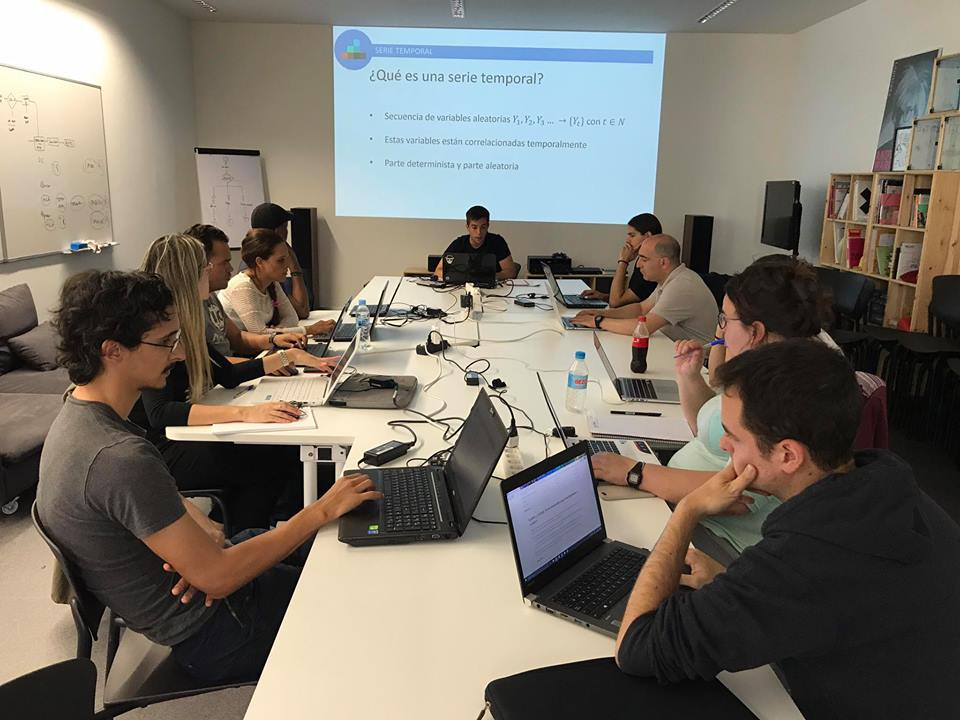
\includegraphics[scale = 0.3]{Images/taller-2.jpg}}
\end{figure}

\end{frame}

%------------------------------------------------

\begin{frame}

\begin{center}
\Huge{Gracias por su atención}
\end{center}

\end{frame}

\end{document} 